\documentclass[10pt,a4paper]{article}
\usepackage[pdftex]{graphicx}
\usepackage{graphicx}
\usepackage{amsmath}
\usepackage{listings}
\usepackage{url}
\usepackage[left=20mm, top=0in]{geometry}
\date{}
\begin{document}
\title{Assignment No 5 : Laplace Equation}
\author{JAGAN M J EE20B047}
\maketitle


\section{AIM}

Aim is to solve the Laplace's Equation in $2$-Dimensions and plot the necessary graphs

\section{Solution to Laplace's Equation}
Laplace's equation in 2-dimensions can  be written in Cartesian coordinates as 





Approximate solution for the above equation for a 2-dimensional grid of points would be 
\begin{equation}
 \frac{\partial^{2} \phi}{\partial x^{2}}+ \frac{\partial^{2} \phi}{\partial y^{2}} = 0
 \end{equation}
This means that the potential at any point is average of the potentials of the neighbouring points

\section{Initial Potential}
The potential of the central circular section is made one and the rest of the region is made zero by the Code 1 in the py code. The required contour plot of the potential region is plotted below with colorbar indicating the magnitude of potential at diferent regions:\newline \newline \newline \newline 

\begin{figure}[!tbh]

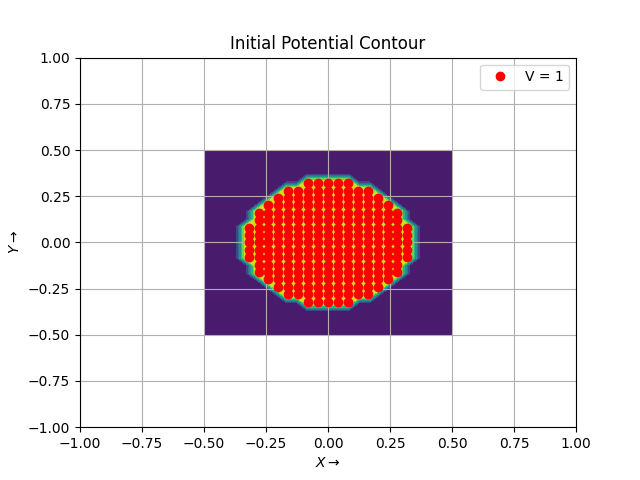
\includegraphics[width = 0.9\textwidth]{1.png}
\caption{Contour plot of initial potential configuration}

\end{figure}


\section{Updating potential to obtain the solution}
We update the values of initial solution by taking the value at each point to be the average of the potential of the neighbouring points and also considering the boundary conditions too. This is done in the the Code 2. A copy of the initial solution is passed to 'oldphi' and the values of the interior ppints are updated by obtaining the average of potentials and potential of the boundaries are taken to be the potential of the next nearest row/column. Also the potential of the central region is also made '1' explicitly. The loop is run several times and the error in the new solution and old solution is compared to stop the iteration. This code takes about 2188 iterations till the error becomes approximately equal to zero

\section{Error estimation}
A graph is plotted between the error and no of iteration taken place both in semilog and loglog scale as shown in below:

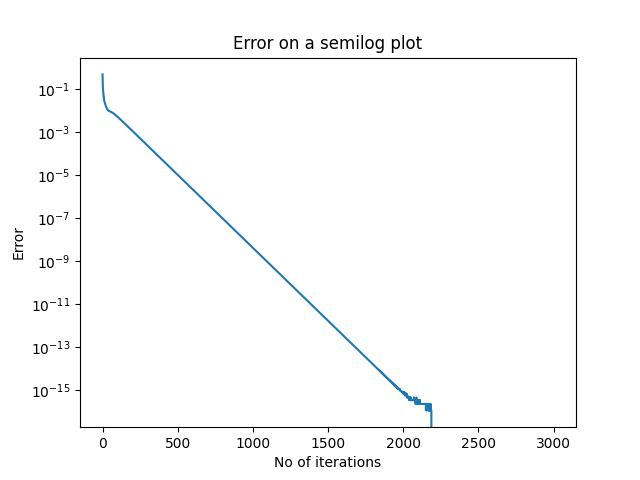
\includegraphics[width = 0.9\textwidth]{2.png}
\newline
For semilog plot, the graph looks like a straight line

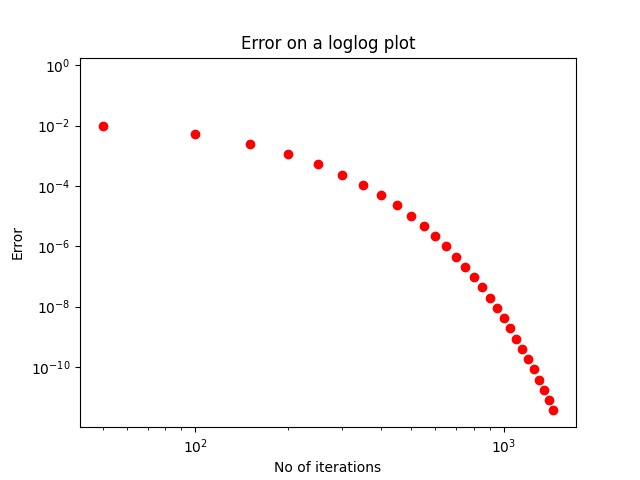
\includegraphics[width = 0.9\textwidth]{3.png}
\newline
For loglog plot , the graph is linear for about 500 iteration and later decays exponentially.
\newline
Next, we find the fit using the least squares approach for iterations from the beginning and also from iterations above 500 and plot them along with the original error plot

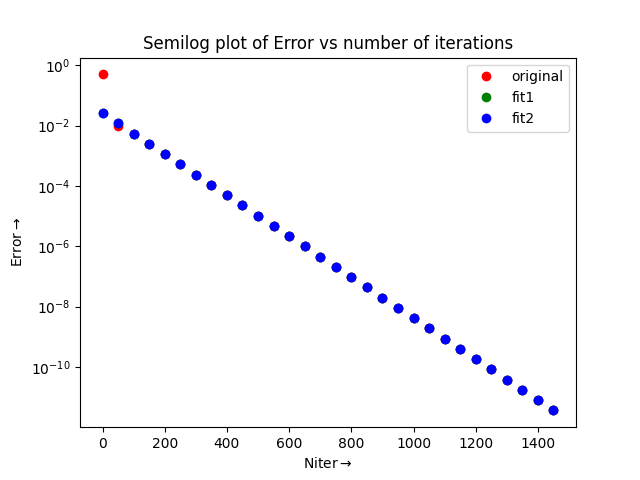
\includegraphics[width = 0.9\textwidth]{4.png}

Both the three plots seems to coincide with each other implying that the error obtained by the least squares approach and the actual error are almost same.
\newline \newline \newline \newline \newline

 \section{Stopping condition}
The upper bound for the error estimated with each iteration is given by \\
\begin{center}
Error = $-\dfrac{A}{B} exp(B(N+0.5))$ 
\end{center}

This error is plotted with no of iterations and the graph is obtained as shown below:
\begin{center}
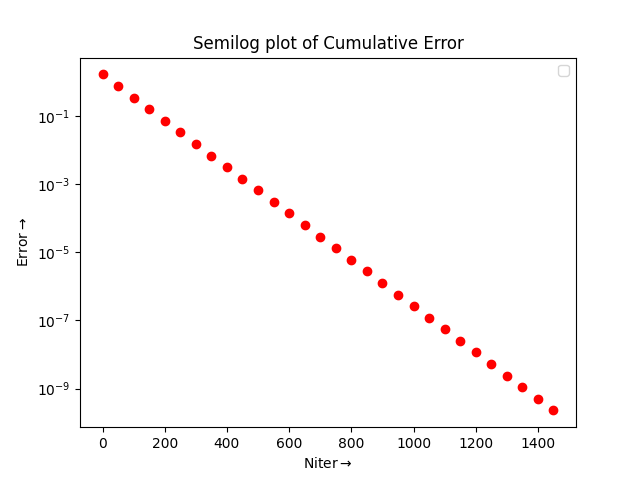
\includegraphics{5.png}
\end{center}
 
\section{Surface plot of potential}

A 3-D plot of the potential is plotted with the help of  function. A total of 2188 iterations took place in plotting the graph

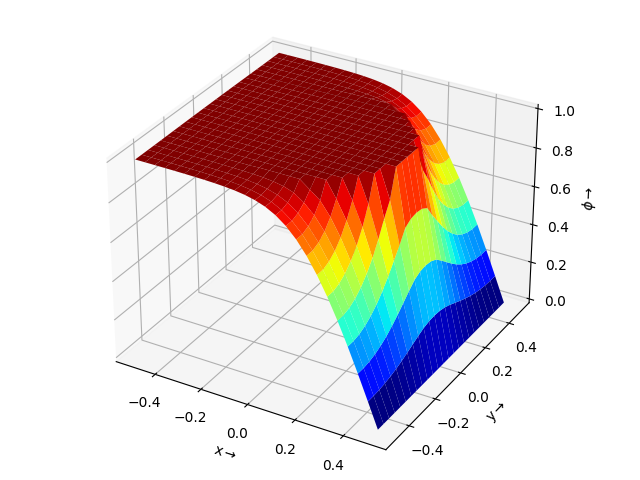
\includegraphics[width = 0.9\textwidth]{6.png}

The contour plot of $\phi$ is obtained using the 'pylab.contour' function.

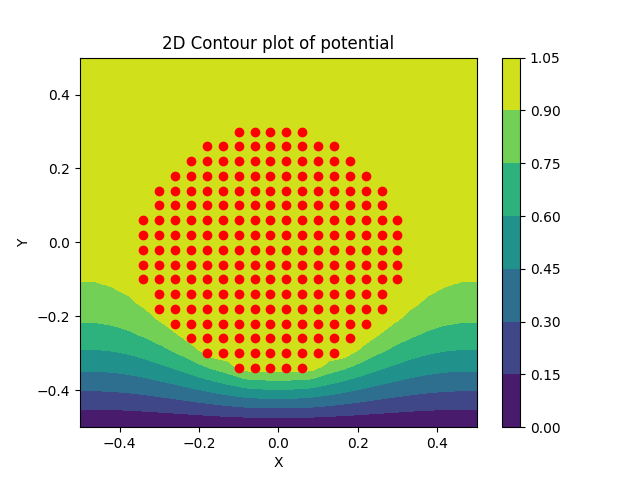
\includegraphics[width = 0.9\textwidth]{7.png}

 \section{Vector plot of currents}

 The currents in the system in Cartesian form can be expressed as :
\begin{equation}
 J_x = -\frac{\partial \phi}{\partial x} 
\end{equation}

\begin{equation}
 J_y = -\frac{\partial \phi}{\partial y} 
\end{equation}
 
 \begin{equation}
 J_{x,ij} = \frac{1}{2}(\phi_{i,j-1} - \phi_{i,j+1}) 
 \end{equation}

\begin{equation}
 J_{y,ij} = \frac{1}{2}(\phi_{i-1,j} - \phi_{i+1,j}) 
\end{equation}

The current density vector is now plotted using the 'quiver'  function. The following plot is obtained :

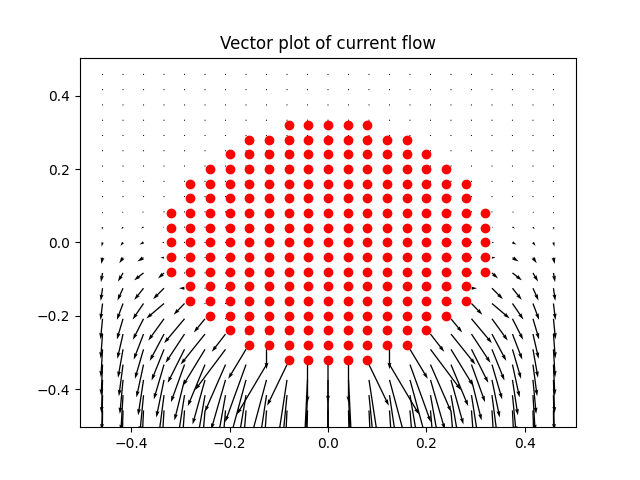
\includegraphics[width = 0.9\textwidth]{8.png}

From the current density plot, we notice that hardly any current flows through the top part of the wire. With a little thought, we observe that the lower surface being grounded, the easiest way for charge carriers to flow from the electrode would be directly through the lower half of the wire, thus avoiding a longer,  more resistive path through the top half of the wire.

 \section{Conclusion}

Using a finite differentiation approximation, we have found a solution to Laplace's equation. The error is seen to decay at a highly gradual pace. On analysing the quiver plot of the currents, it was noticed that the current was mostly restricted to the bottom of the wire, and was perpendicular to the surface of the electrode and the conductor. 
\end{document}